\documentclass{article}
\usepackage{fancyhdr}
\usepackage{ctex}
\usepackage[a4paper, body={18cm,22cm}]{geometry}
\usepackage{amsmath,amssymb,amstext,wasysym,enumerate,graphicx}
\usepackage{float,abstract,booktabs,indentfirst,amsmath}
\usepackage{multirow}
\usepackage{enumitem}
\usepackage{xcolor}
\usepackage{tabularx}
\usepackage[most]{tcolorbox}
\usepackage{accsupp}
\usepackage[bottom]{footmisc}
\usepackage{subcaption}
\usepackage{logicproof}
% \usepackage[backend=biber,style=numeric]{biblatex}
\usepackage[xetex]{hyperref}
\usepackage{fontspec}
\usepackage{listingsutf8}
\usepackage{xcolor}
\usetikzlibrary{arrows.meta}
\newcommand\emptyaccsupp[1]{\BeginAccSupp{ActualText={}}#1\EndAccSupp{}}
\setlength{\parindent}{2em}
\setmonofont{Consolas}
\setCJKmonofont{黑体}
% \setmainfont{Times New Roman}
\hypersetup{CJKbookmarks=true,colorlinks=true,citecolor=blue,%
            linkcolor=blue,urlcolor=blue,bookmarksnumbered=true,%
            bookmarksopen=true,breaklinks=true}
\lstset{
    % language = C,
    inputencoding=utf8,
    extendedchars=false,
    showstringspaces=false,
    xleftmargin = 3em,xrightmargin = 3em, aboveskip = 1em,
	backgroundcolor = \color{white}, % 背景色
	basicstyle = \small\ttfamily, % 基本样式 + 小号字体
	rulesepcolor= \color{gray}, % 代码块边框颜色
	breaklines = true, % 代码过长则换行
	numbers = left, % 行号在左侧显示
	numberstyle=\emptyaccsupp,
    numbersep = 14pt, 
    keywordstyle=\color{purple}\bfseries, % 关键字颜色
    commentstyle =\color{red!50!green!50!blue!60}, % 注释颜色
    stringstyle = \color{red}, % 字符串颜色
    morekeywords={ASSERT, int64_t, uint32_t},
	% frame = shadowbox, % 用(带影子效果)方框框住代码块
	frame = single, % 用(带影子效果)方框框住代码块
	showspaces = false, % 不显示空格
	columns = fixed, % 字间距固定
  framesep=1em
} 
\lstset{
    sensitive=true,
    moreemph={ASSERT, NULL}, emphstyle=\color{red}\bfseries,
    moreemph=[2]{int64_t, uint32_t, tid_t, uint8_t, int16_t, uint16_t, int32_t, size_t}, emphstyle=[2]\color{purple}\bfseries,
    showspaces = false, % 不显示空格
    }

\raggedbottom

\title{\heiti\textbf{机器学习实践报告}}
\author{第六次实验 \\ 
武泽恺 10225101429
}
\date{2025年12月15日}



\begin{document}
\maketitle

\section{实验目的}
\begin{itemize}
  \item 理解集成学习中 Bagging 与 Boosting 的基本思想。
  \item 掌握 Bagging、AdaBoost 和 GBDT 在分类与回归问题中的应用。
  \item 比较不同集成学习方法的性能差异。
\end{itemize}

\section{实验环境}
\begin{itemize}
    \item Python 3.11.7
    \item 主要库：
    \begin{itemize}
        \item \texttt{scikit-learn}
        \item \texttt{numpy}
        \item \texttt{matplotlib}
    \end{itemize}
\end{itemize}

\section{实验内容与步骤}

\subsection{MNIST 数据集分类实验}

MNIST 数据集包含 0–9 的手写数字图像，每张图片大小为 $28\times28$。实验中将像素值归一化至 $[0,1]$，并划分训练集与测试集。

\subsubsection{Bagging + 决策树}

采用 BaggingClassifier，以决策树作为基分类器，通过对训练样本进行有放回抽样，训练多个基模型并进行投票。

我们可以得到：

\begin{itemize}
    \item Accuracy: 0.895
    \item F1-score: 0.8939272815739792
\end{itemize}

\begin{table}[H]
    \centering
    \caption{MNIST - Bagging 分类性能报告}
    \label{tab:bagging_mnist_report}
    \begin{tabular}{cccccc}
      \toprule
      类别 & Precision & Recall & F1-score & 样本数 \\
      \midrule
      0 & 0.88 & 0.95 & 0.91 & 146 \\
      1 & 0.95 & 0.98 & 0.96 & 177 \\
      2 & 0.87 & 0.87 & 0.87 & 151 \\
      3 & 0.91 & 0.87 & 0.89 & 167 \\
      4 & 0.91 & 0.80 & 0.85 & 143 \\
      5 & 0.85 & 0.88 & 0.86 & 154 \\
      6 & 0.94 & 0.90 & 0.92 & 177 \\
      7 & 0.97 & 0.93 & 0.95 & 155 \\
      8 & 0.87 & 0.87 & 0.87 & 167 \\
      9 & 0.81 & 0.89 & 0.85 & 163 \\
      \midrule
      Accuracy & \multicolumn{3}{c}{0.90} & 1600 \\
      Macro\,avg & 0.90 & 0.89 & 0.89 & 1600 \\
      Weighted\,avg & 0.90 & 0.90 & 0.90 & 1600 \\
      \bottomrule
    \end{tabular}
  \end{table}

\begin{figure}[H]
\centering
\begin{minipage}{0.45\textwidth}
    \centering
    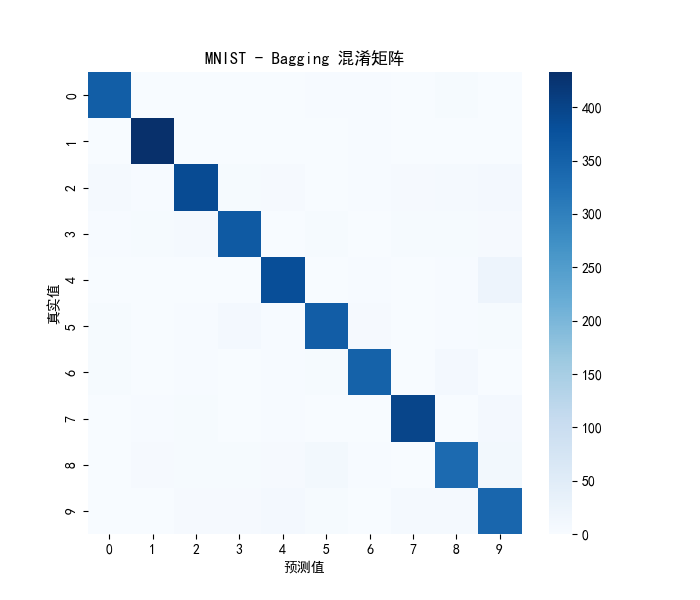
\includegraphics[width=\linewidth]{1.png}
    \caption{MNIST – Bagging 混淆矩阵}
    \label{fig:bagging_mnist_left}
\end{minipage}\hfill
\begin{minipage}{0.45\textwidth}
    \centering
    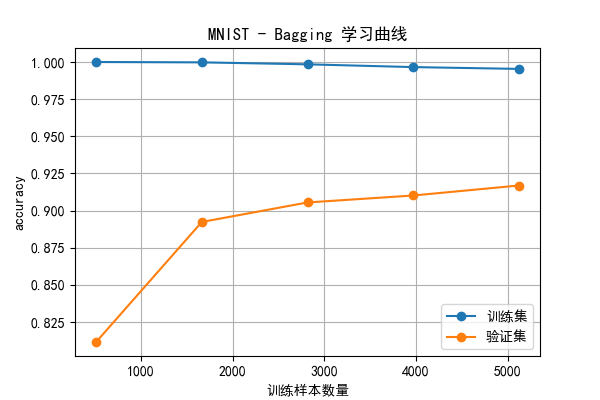
\includegraphics[width=\linewidth]{2.png}
    \caption{MNIST – Bagging 学习曲线}
    \label{fig:bagging_mnist_right}
\end{minipage}
\end{figure}

\subsubsection{AdaBoost}

AdaBoost 通过不断调整样本权重，使模型更加关注分类错误的样本，提高整体性能。

我们可以得到：

\begin{itemize}
    \item Accuracy: 0.755625
    \item F1-score: 0.7538816767416859
\end{itemize}

\begin{table}[H]
    \centering
    \caption{MNIST - AdaBoost 分类性能报告}
    \label{tab:metrics2}
    \begin{tabular}{cccccc}
      \toprule
      类别 & Precision & Recall & F1-score & 样本数 \\
      \midrule
      0 & 0.89 & 0.77 & 0.82 & 141 \\
      1 & 0.93 & 0.95 & 0.94 & 190 \\
      2 & 0.60 & 0.59 & 0.59 & 172 \\
      3 & 0.77 & 0.62 & 0.68 & 162 \\
      4 & 0.86 & 0.74 & 0.79 & 162 \\
      5 & 0.61 & 0.64 & 0.63 & 143 \\
      6 & 0.74 & 0.77 & 0.76 & 141 \\
      7 & 0.90 & 0.82 & 0.86 & 160 \\
      8 & 0.63 & 0.84 & 0.72 & 157 \\
      9 & 0.70 & 0.78 & 0.74 & 172 \\
      \midrule
      Accuracy & \multicolumn{3}{c}{0.76} & 1600 \\
      Macro\,avg & 0.76 & 0.75 & 0.75 & 1600 \\
      Weighted\,avg & 0.77 & 0.76 & 0.76 & 1600 \\
      \bottomrule
    \end{tabular}
  \end{table}

\begin{figure}[H]
    \centering
    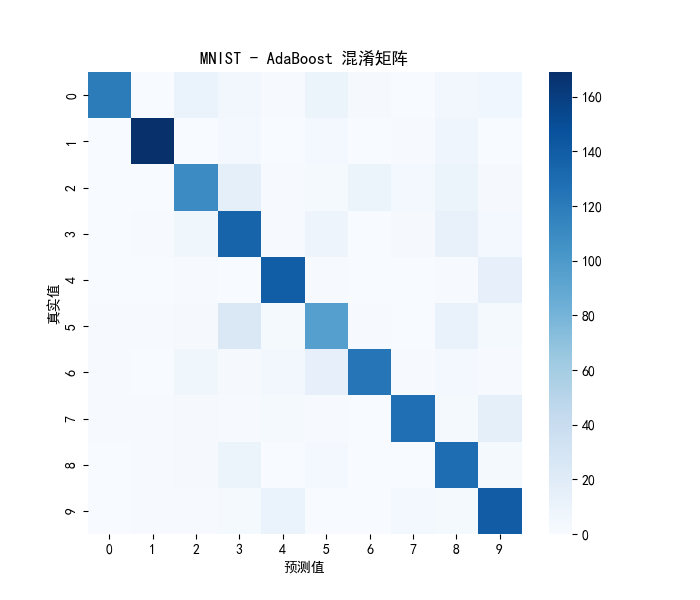
\includegraphics[width=0.4\textwidth]{3.png}
    \caption{MNIST - AdaBoost 混淆矩阵}
    \label{fig:bagging_mnist_confusion_matrix}
\end{figure}


\subsubsection{Gradient Boosting}

GBDT 采用前向分步算法，每一棵新树拟合前一轮的残差。

我们可以得到：

\begin{itemize}
    \item Accuracy: 0.869375
    \item F1-score: 0.8687298946695317
\end{itemize}

\begin{table}[H]
    \centering
    \caption{MNIST - GBDT 分类性能报告}
    \label{tab:metrics3}
    \begin{tabular}{cccccc}
      \toprule
      类别 & Precision & Recall & F1-score & 样本数 \\
      \midrule
      0 & 0.95 & 0.94 & 0.94 & 173 \\
      1 & 0.91 & 0.97 & 0.94 & 160 \\
      2 & 0.86 & 0.84 & 0.85 & 167 \\
      3 & 0.88 & 0.79 & 0.83 & 180 \\
      4 & 0.87 & 0.90 & 0.89 & 155 \\
      5 & 0.83 & 0.84 & 0.84 & 121 \\
      6 & 0.87 & 0.89 & 0.88 & 133 \\
      7 & 0.90 & 0.88 & 0.89 & 178 \\
      8 & 0.83 & 0.78 & 0.81 & 180 \\
      9 & 0.78 & 0.87 & 0.82 & 153 \\
      \midrule
      Accuracy & \multicolumn{3}{c}{0.87} & 1600 \\
      Macro\,avg & 0.87 & 0.87 & 0.87 & 1600 \\
      Weighted\,avg & 0.87 & 0.87 & 0.87 & 1600 \\
      \bottomrule
    \end{tabular}
  \end{table}

  \begin{figure}[H]
    \centering
    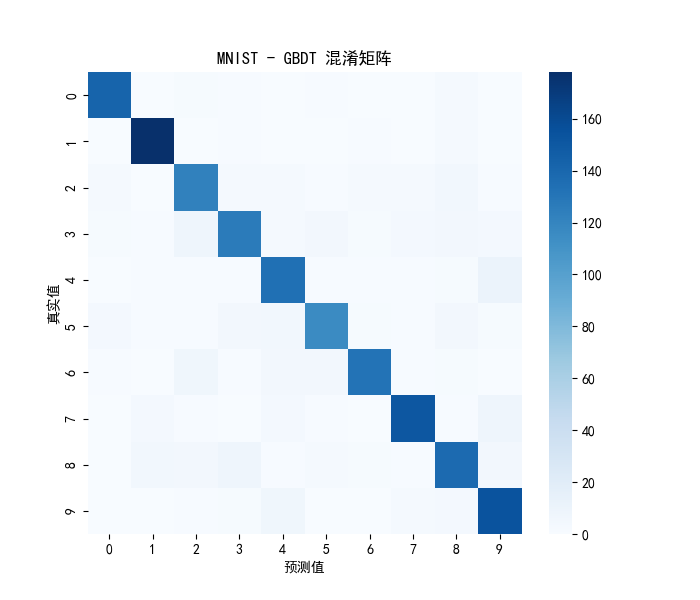
\includegraphics[width=0.4\textwidth]{4.png}
    \caption{MNIST - GBDT 混淆矩阵}
    \label{fig:bagging_mnist_confusion_matrix}
\end{figure}

通过上述实验结果可以看出，不同集成学习方法在 MNIST 多分类任务上表现各有特点。Bagging 方法因为能够降低基学习器的方差，整体准确率较高，F1-score 达到 0.89，尤其对高方差模型如决策树提升显著。AdaBoost 虽然在部分类别上表现突出（如对“1”类别的 recall 达到 0.95），但整体准确率和 F1-score 略低，说明其更敏感于噪声数据，部分类别召回率和精度表现不均。GBDT 综合了前述两者优势，能够有效拟合复杂数据，准确率和 F1-score 均接近 Bagging，同时在多数类别上表现均衡，具有较强泛化能力。

\subsection{California Housing 回归实验}

California Housing 数据集用于预测房价中位数，采用 RMSE、MAE 和 $R^2$ 作为评估指标。

\subsubsection{Bagging + 决策树}

我们可以得到：

\begin{itemize}
    \item RMSE: 0.5128643938556334
    \item MAE: 0.3533773875483425
    \item $R^2$: 0.7992764924138424
\end{itemize}

\begin{figure}[H]
    \centering
    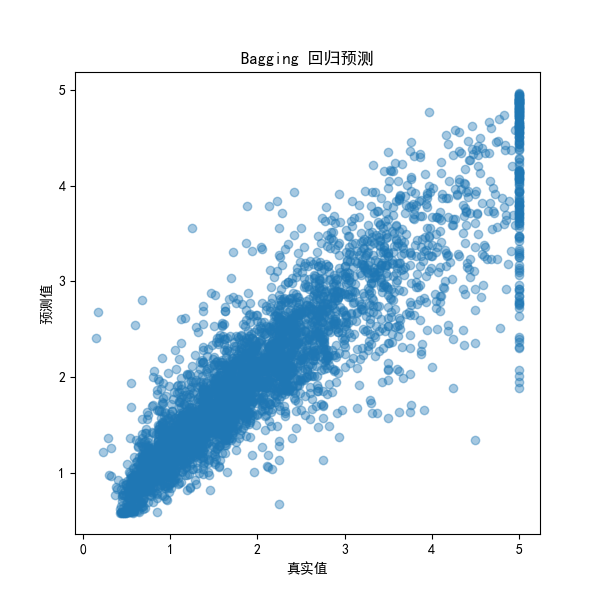
\includegraphics[width=0.4\textwidth]{5.png}
    \caption{California Housing - Bagging 散点图}
    \label{fig:bagging_mnist_confusion_matrix}
\end{figure}

\subsubsection{AdaBoost}

我们可以得到：

\begin{itemize}
    \item RMSE: 0.7393227183231676
    \item MAE: 0.6155107462521047
    \item $R^2$: 0.5828797795917773
\end{itemize}

\begin{figure}[H]
    \centering
    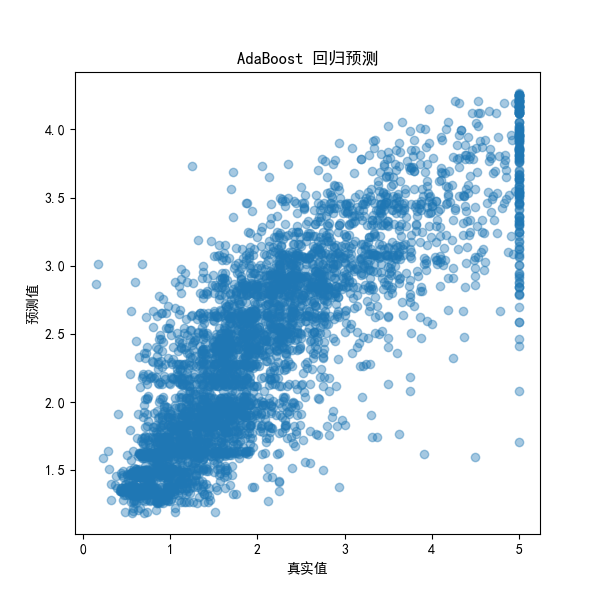
\includegraphics[width=0.4\textwidth]{6.png}
    \caption{California Housing - AdaBoost 散点图}
    \label{fig:bagging_mnist_confusion_matrix}
\end{figure}

\subsubsection{Gradient Boosting}

我们可以得到：

\begin{itemize}
    \item RMSE: 0.5396427492600185
    \item MAE: 0.368997422307243
    \item $R^2$: 0.7777683901251662
\end{itemize}

\begin{figure}[H]
    \centering
    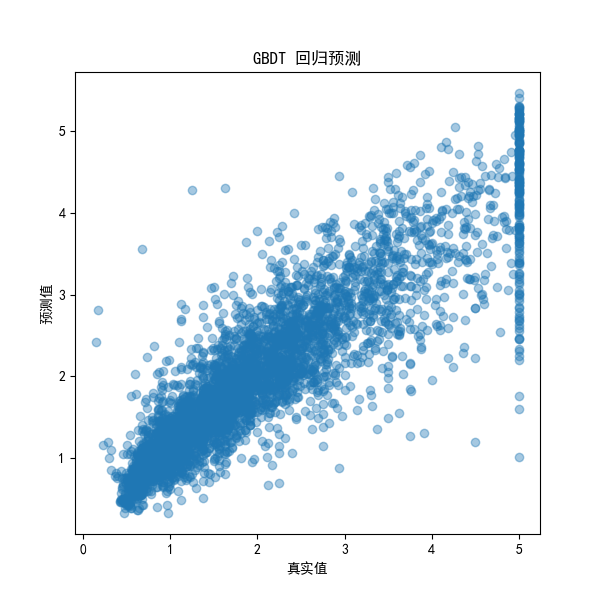
\includegraphics[width=0.4\textwidth]{7.png}
    \caption{California Housing - GBDT 散点图}
    \label{fig:bagging_mnist_confusion_matrix}
\end{figure}

从上述实验结果可以看出，Bagging 在本任务中表现最优，GBDT 次之，AdaBoost 效果一般。这说明当基学习器本身能力较强（如回归树）且数据集中存在一定噪声时，Bagging 通过集成降方差可以获得更好的泛化效果，而 Boosting 方法在此场景下提升有限甚至容易过拟合噪声。

\section{实验总结}

通过本实验，我深入理解了集成学习方法在分类与回归问题中的优势。Bagging 更适合高方差模型，而 Boosting 在复杂任务中具有更强的拟合能力。 

\newpage
\appendix
\section{完整代码}

\begin{lstlisting}[language=Python]
from matplotlib import rcParams
import matplotlib.pyplot as plt
import numpy as np
import seaborn as sns
from sklearn.datasets import fetch_california_housing, fetch_openml
from sklearn.ensemble import (
    AdaBoostClassifier,
    AdaBoostRegressor,
    BaggingClassifier,
    BaggingRegressor,
    GradientBoostingClassifier,
    GradientBoostingRegressor,
)
from sklearn.metrics import (
    accuracy_score,
    classification_report,
    confusion_matrix,
    f1_score,
    mean_absolute_error,
    mean_squared_error,
    r2_score,
)
from sklearn.model_selection import train_test_split
from sklearn.model_selection import learning_curve
from sklearn.tree import DecisionTreeClassifier, DecisionTreeRegressor

rcParams["font.sans-serif"] = ["SimHei"]
rcParams["axes.unicode_minus"] = False


def load_mnist(sample_size=8000):
    mnist = fetch_openml("mnist_784", version=1, as_frame=False)
    X = mnist.data
    y = mnist.target.astype(int)

    idx = np.random.choice(len(X), sample_size, replace=False)
    X = X[idx] / 255.0
    y = y[idx]

    return train_test_split(X, y, test_size=0.2, random_state=42)


def plot_learning_curve(estimator, X, y, title, scoring, cv=5, train_sizes=np.linspace(0.1, 1.0, 5)):
    train_sizes, train_scores, val_scores = learning_curve(
        estimator, X, y, cv=cv, scoring=scoring, train_sizes=train_sizes, n_jobs=-1
    )

    train_mean = np.mean(train_scores, axis=1)
    val_mean = np.mean(val_scores, axis=1)

    plt.figure(figsize=(6, 4))
    plt.plot(train_sizes, train_mean, "o-", label="训练集")
    plt.plot(train_sizes, val_mean, "o-", label="验证集")
    plt.title(title)
    plt.xlabel("训练样本数量")
    plt.ylabel(scoring)
    plt.legend()
    plt.grid()
    plt.show()


def bagging_mnist():
    X_train, X_test, y_train, y_test = load_mnist()

    model = BaggingClassifier(
        estimator=DecisionTreeClassifier(max_depth=10),
        n_estimators=50,
        max_features=0.8,
        n_jobs=-1,
        random_state=42,
    )

    model.fit(X_train, y_train)
    y_pred = model.predict(X_test)

    print("Accuracy:", accuracy_score(y_test, y_pred))
    print("F1-score:", f1_score(y_test, y_pred, average="macro"))

    cm = confusion_matrix(y_test, y_pred)
    plt.figure(figsize=(7, 6))
    sns.heatmap(cm, cmap="Blues", fmt="d")
    plt.title("MNIST - Bagging 混淆矩阵")
    plt.xlabel("预测值")
    plt.ylabel("真实值")
    plt.show()

    print(classification_report(y_test, y_pred))

    plot_learning_curve(model, X_train, y_train, "MNIST - Bagging 学习曲线", "accuracy")


def adaboost_mnist():
    X_train, X_test, y_train, y_test = load_mnist()

    model = AdaBoostClassifier(
        estimator=DecisionTreeClassifier(max_depth=2),
        n_estimators=100,
        learning_rate=0.5,
        random_state=42,
    )

    model.fit(X_train, y_train)
    y_pred = model.predict(X_test)

    print("Accuracy:", accuracy_score(y_test, y_pred))
    print("F1-score:", f1_score(y_test, y_pred, average="macro"))

    cm = confusion_matrix(y_test, y_pred)
    plt.figure(figsize=(7, 6))
    sns.heatmap(cm, cmap="Blues", fmt="d")
    plt.title("MNIST - AdaBoost 混淆矩阵")
    plt.xlabel("预测值")
    plt.ylabel("真实值")
    plt.show()

    print(classification_report(y_test, y_pred))


def gbdt_mnist():
    X_train, X_test, y_train, y_test = load_mnist()

    model = GradientBoostingClassifier(
        n_estimators=50, learning_rate=0.1, max_depth=2, random_state=42
    )

    model.fit(X_train, y_train)
    y_pred = model.predict(X_test)

    print("Accuracy:", accuracy_score(y_test, y_pred))
    print("F1-score:", f1_score(y_test, y_pred, average="macro"))

    cm = confusion_matrix(y_test, y_pred)
    plt.figure(figsize=(7, 6))
    sns.heatmap(cm, cmap="Blues", fmt="d")
    plt.title("MNIST - GBDT 混淆矩阵")
    plt.xlabel("预测值")
    plt.ylabel("真实值")
    plt.show()

    print(classification_report(y_test, y_pred))


def load_housing():
    housing = fetch_california_housing()
    X = housing.data
    y = housing.target
    return train_test_split(X, y, test_size=0.2, random_state=42)


def bagging_housing():
    X_train, X_test, y_train, y_test = load_housing()

    model = BaggingRegressor(
        estimator=DecisionTreeRegressor(max_depth=10),
        n_estimators=100,
        max_features=0.8,
        n_jobs=-1,
        random_state=42,
    )

    model.fit(X_train, y_train)
    y_pred = model.predict(X_test)

    rmse = np.sqrt(mean_squared_error(y_test, y_pred))
    mae = mean_absolute_error(y_test, y_pred)
    r2 = r2_score(y_test, y_pred)

    print("RMSE:", rmse)
    print("MAE:", mae)
    print("R2:", r2)

    plt.figure(figsize=(6, 6))
    plt.scatter(y_test, y_pred, alpha=0.4)
    plt.xlabel("真实值")
    plt.ylabel("预测值")
    plt.title("Bagging 回归预测")
    plt.show()


def adaboost_housing():
    X_train, X_test, y_train, y_test = load_housing()

    model = AdaBoostRegressor(
        estimator=DecisionTreeRegressor(max_depth=4),
        n_estimators=200,
        learning_rate=0.1,
        random_state=42,
    )

    model.fit(X_train, y_train)
    y_pred = model.predict(X_test)

    print("RMSE:", np.sqrt(mean_squared_error(y_test, y_pred)))
    print("MAE:", mean_absolute_error(y_test, y_pred))
    print("R2:", r2_score(y_test, y_pred))

    plt.figure(figsize=(6, 6))
    plt.scatter(y_test, y_pred, alpha=0.4)
    plt.xlabel("真实值")
    plt.ylabel("预测值")
    plt.title("AdaBoost 回归预测")
    plt.show()


def gbdt_housing():
    X_train, X_test, y_train, y_test = load_housing()

    model = GradientBoostingRegressor(
        n_estimators=200, learning_rate=0.05, max_depth=3, random_state=42
    )

    model.fit(X_train, y_train)
    y_pred = model.predict(X_test)

    print("RMSE:", np.sqrt(mean_squared_error(y_test, y_pred)))
    print("MAE:", mean_absolute_error(y_test, y_pred))
    print("R2:", r2_score(y_test, y_pred))

    plt.figure(figsize=(6, 6))
    plt.scatter(y_test, y_pred, alpha=0.4)
    plt.xlabel("真实值")
    plt.ylabel("预测值")
    plt.title("GBDT 回归预测")
    plt.show()


if __name__ == "__main__":
    bagging_mnist()
    adaboost_mnist()
    gbdt_mnist()

    bagging_housing()
    adaboost_housing()
    gbdt_housing()
    
\end{lstlisting}

\end{document}